\documentclass[12.5pt]{scrartcl}
\usepackage[automark]{scrlayer-scrpage}
\clearpairofpagestyles
\ihead{\textsc{Functional Programming}}
\ohead{Su Xiaotian -- Clean Music Generator}
\renewcommand{\headfont}{\small}
\cfoot{\thepage}

\usepackage[T1]{fontenc}
\usepackage{mathtools}
\usepackage{amsfonts}
\usepackage{amsmath}
\usepackage{tabu}
\usepackage{amssymb,amsthm}
\usepackage{stuki}
\usepackage{tikz-uml}
\usepackage{graphicx}
\usepackage{geometry}
\usepackage{float}
\usepackage{diagbox}
\usepackage[utf8]{inputenc}

\DeclareMathOperator*{\Max}{Max}
\setlength{\parskip}{.5em}
\setlength{\parindent}{0pt}
\geometry{footskip=3.5cm}

\begin{document}
\begin{titlepage}
	\begin{center}
		\vspace*{2cm}
		
		\Huge
		\textbf{Clean Music Generator}
		
		\vspace{0.8cm}
		\LARGE
		\textbf{Reading from MIDI file}
		
		\vspace{1.8cm}
		
		\textbf{Su Xiaotian}\\
		\textit{suxiaotian31@gmail.com}	
		\vfill
		
		\includegraphics[width=0.3\textwidth]{ELTE_logo}
		
		\Huge
		\today	
	\end{center}
\end{titlepage}

\tableofcontents
\newpage

\setlength{\parskip}{5pt}
\section{Background Information of MIDI File}
\subsection{A general information of MIDI file}
\subsubsection{What are MIDI files}
MIDI is short for Musical Instrument Digital Interface which related audio devices for playing, editing and recording music.\\
The MIDI file is just a stream of numbers, each of which is in the range from 0 to 255.\\
The bytes order are big endian.\\
\subsubsection{What are in the MIDI files}
MIDI files are consists of chunks.There are two types of chunks.\\
\renewcommand{\arraystretch}{2.0}
\begin{center}
	\begin{tabu}{|l|m{5em}|m{5em}|m{13em}|}
	   \hline
	   \diagbox[width=7.85em]{\bfseries type}{\bfseries structure}
	        & type \newline (4 bytes)
	        & length \newline (4 bytes) 
	        & data \newline (variable length of bytes) \\
		\hline
		Header Chunk & MThd & 6 & <format><tracks><division>\\ 
		\hline
		Track Chunk & MTrk & <length> & <delta\_time><events>... \\  
		\hline
	\end{tabu}
\end{center}
length : length in bytes of the chunk data part

\subsection{Data In Header Chunk} 
\subsubsection{Format}
    \begin{itemize}
     \item format 0 : a header chunk $+$ a single track chunk.  \\
        \-\hspace{4.7em}The single track chunk contains all the note and tempo information.
     \item format 1 : a header chunk $+$ one or more track chunks.  \\
        \-\hspace{4.7em}All tracks being played simultaneously.
     \item format 2 : a header chunk $+$ one or more track chunks.  \\
        \-\hspace{4.7em}Each track represents an independent sequence.
    \end{itemize}
\subsubsection{Tracks}
The number of track chunks contained in MIDI file.

\subsubsection{Division}
The default unit of delta-time for this MIDI file.


\subsection{Data In Track Chunk}
\subsubsection{Delta Time}
    \begin{itemize}
        \item a time value which specifies the duration between two events
        \item not optional
        \item 0 is a valid delta time
    \end{itemize}
    
\subsubsection{Events}
The default unit of delta-time for this MIDI file.
\begin{itemize}
 \item midi events : any MIDI Channel message.
    \begin{itemize}
        \item Channel Voice messages
        \item Channel Mode messages
    \end{itemize}
 \item sysex(system exclusive) events : include messages other than MIDI Channel.
 \item meta events : used for things like track-names, lyrics and cue-points, etc.
\end{itemize}



\section{Challenges}
Unlike regular audio files like MP3 or WAV files, MIDI files don't contain actual audio data and are therefore much smaller in size.In this case,they are more compact and this make it more difficult to parse it since there are a lot of information to extract and store.\\
\subsection{Variable length of delta time}
\subsubsection{Explanation}
Delta time is represented by a time value which is a measurement of the time to wait before playing the next message in the stream of MIDI file data.Time values are stored as Variable Length Values (VLV:a number with a variable width).
\subsubsection{Calculation}
Each byte of delta time is consist of two parts: 1 continuation bit and 7 data bits. The highest-order bit is set to 1 if it needs to read the next byte, set to 0 if this byte is the last one in VLV.
\paragraph{Steps:}
To get an integer number represented by a VLV
\begin{enumerate}
    \item convert the first byte in VLV to integer
        \begin{itemize}
            \item if it is greater than 128, put it into a list and read next byte recursively
            \item if not, just put this byte into a list and end the recursion
        \end{itemize}
    \item convert the list of bytes into one integer number
    \item return not only an integer of delta time but also the length of byte of it
\end{enumerate}

\paragraph{Graph Illustration}
\begin{center}
\renewcommand{\arraystretch}{0.9}% Tighter
    \begin{tabular}{|c|c|c|c|c|c|c|c|}
        \hline
        1&...&...&...&...&...&...&...\\[1pt]
        \hline
    \end{tabular}
    %\-\hspace{3em}
    \begin{tabular}[height=0.3em]{|c|c|c|c|c|c|c|c|}
        \hline
        0&...&...&...&...&...&...&...\\
        \hline
    \end{tabular}
\end{center}
\subsection{Variable length of events in track chunk}
\subsubsection{Explanation}
There are three main different kinds of events that can occur in track chunk, each type has different number of bytes to store the information.We are not able to know the length of each specific event until we reach its status byte which stores the information indicating what type it is.
\begin{center}
	\begin{tabu}{|l|m{7em}|m{4em}|m{4em}|m{4em}|}
	    \hline
	    \diagbox[width=7.8em]{\bfseries event type}{\bfseries structure} 
	    & status byte & byte2 & byte3 & byte4 \\
        \hline
		midi events & 0x8n - 0xEn & data & (data) & $-$\\ 
		\hline
		sysex events & 0xF0 and 0xF7 & length & data & $-$\\  
		\hline
		meta events & 0xFF & type & length & data \\  
		\hline
	\end{tabu}
\end{center}
\paragraph{Running Status: }
Different types of events already make it hard to parse information, in addition to that, the midi events use  a data-thinning technique which is running status.
If the first (status) byte is less than 128 (hex 80) which implies that running status is in effect, and that this byte is actually the first data byte (the status carrying over from the previous MIDI event). This can only be the case if the immediately previous event is also a MIDI event, because system exclusive events and meta events interrupt (clear) running status.

\subsubsection{Extration}

\section{Solutions}
\subsection{Type used}
the length of track chunk is useful since it is not only help for processing normal chunks but also make it easier to deal with unexpected chunk types -- just by skiping that amount of byte then we can continue to process next chunk.

\subsection{Events handled so far}
\begin{center}
	\begin{tabu} to 1.15\textwidth {|m{4.5em}|m{2.5em}|m{4.5em}|m{11em}|m{4em}|}
	    \hline
	    event type & \multicolumn{2}{l|}{status byte} & byte2 & byte3 \\
        \hline
        Note On & 0x8 & Channel & Note Number(frequency) & velocity \\ 
		\hline
		Note Off & 0x9 & Channel & Note Number(frequency) & velocity \\  
		\hline
	\end{tabu}
\end{center}

\subsection{Functions Created}

\subsubsection{Graph Illustration}
\begin{figure}[H]
	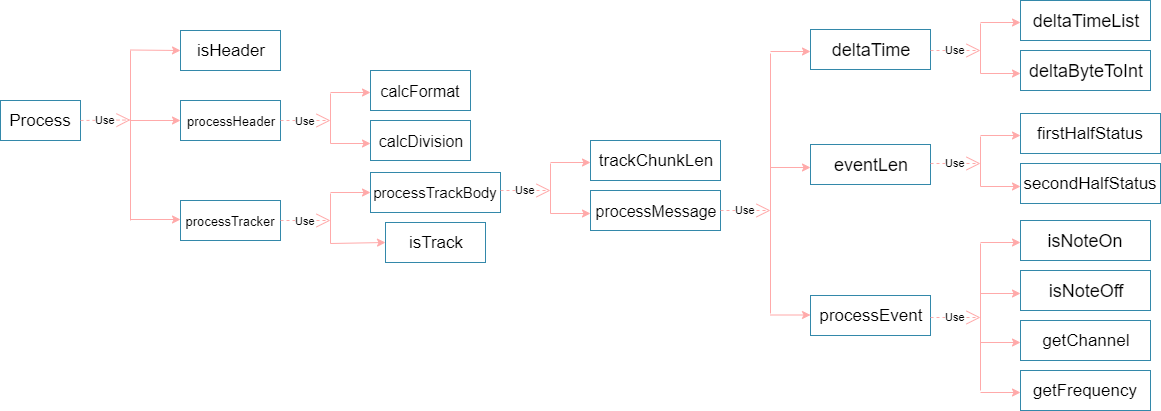
\includegraphics[width=1\textwidth]{functions.png}
\end{figure}

\subsubsection{Detailed explanation}
\textbf{process:}
Parsing MIDI file from scratch,accept a list of Char(i.e.bytes) and give back a\textit{ Info }record which contains information about header chunk and track chunks.
\begin{itemize}
	\item \textbf{isHeader:}take the first four elements of a list of bytes and see if it is the type of header chunk which is "MThd".
\end{itemize}

\textbf{processHeader:}
The first six bytes of the list give information about\textit{ format },number of track chunks in this file and\textit{ division }.We need to store the first and third value in the\textit{ HeadInfo }record.
\begin{itemize}
	\item \textbf{calcFormat:}turn the bytes representation to integer information.
	\item \textbf{calcDivision:}turn the bytes representation to integer information.
\end{itemize}

\textbf{processTrack:}use\textit{ isTrack }function to see if we are now at the beginning of a track chunk,if it gives back true then we drop the fist 4 element which contain the information of chunk type and then

\begin{itemize}
	\item \textbf{isTrack:}take the first four elements of given list of bytes and see if it is the type of track chunk which is "MTrk".
\end{itemize}

\textbf{processTrackBody:}
\begin{itemize}
	\item \textbf{trackChunkLen:}turn the bytes representation to integer information.
\end{itemize}

\textbf{processMessage:}turn the bytes representation to integer information.
\subsection{Testing}

\section{Resources}
https://en.wikipedia.org/wiki/MIDI  \\
https://www.csie.ntu.edu.tw/~r92092/ref/midi/   \\
http://somascape.org/midi/tech/spec.html    \\
http://www.ccarh.org/courses/253/handout/vlv/   \\
http://somascape.org/midi/tech/mfile.html   \\

\end{document}